%%%%%%%%%%%%%%%%%%%%%%%%%%%%%%%%%%%%%%%%
% Wenneker Assignment
% LaTeX Template
% Version 2.0 (12/1/2019)
%
% This template originates from:
% http://www.LaTeXTemplates.com
%
% Authors:
% Vel (vel@LaTeXTemplates.com)
% Frits Wenneker
%
% License:
% CC BY-NC-SA 3.0 (http://creativecommons.org/licenses/by-nc-sa/3.0/)
% 
%%%%%%%%%%%%%%%%%%%%%%%%%%%%%%%%%%%%%%%%%

%----------------------------------------------------------------------------------------
%	PACKAGES AND OTHER DOCUMENT CONFIGURATIONS
%----------------------------------------------------------------------------------------

\documentclass[11pt]{scrartcl} % Font size

%%%%%%%%%%%%%%%%%%%%%%%%%%%%%%%%%%%%%%%
% Wenneker Assignment
% Structure Specification File
% Version 2.0 (12/1/2019)
%
% This template originates from:
% http://www.LaTeXTemplates.com
%
% Authors:
% Vel (vel@LaTeXTemplates.com)
% Frits Wenneker
%
% License:
% CC BY-NC-SA 3.0 (http://creativecommons.org/licenses/by-nc-sa/3.0/)
% 
%%%%%%%%%%%%%%%%%%%%%%%%%%%%%%%%%%%%%%%%%

%----------------------------------------------------------------------------------------
%	PACKAGES AND OTHER DOCUMENT CONFIGURATIONS
%----------------------------------------------------------------------------------------
\usepackage{xcolor}   % for \textcolor
\usepackage{comment}

\usepackage{amsmath, amsfonts, amsthm} % Math packages

\usepackage{listings} % Code listings, with syntax highlighting
\usepackage{verbatim} % Directly from txt file

\usepackage[english]{babel} % English language hyphenation
\usepackage{tikz} 
\usepackage{neuralnetwork} 
\usepackage{graphicx} % Required for inserting images
\graphicspath{{Figures/}{./}} % Specifies where to look for included images (trailing slash required)
\usepackage{setspace}  % allows linespacing changes
\usepackage{tabularx} % for tables

\usepackage{booktabs} % Required for better horizontal rules in tables

\numberwithin{equation}{section} % Number equations within sections (i.e. 1.1, 1.2, 2.1, 2.2 instead of 1, 2, 3, 4)
\numberwithin{figure}{section} % Number figures within sections (i.e. 1.1, 1.2, 2.1, 2.2 instead of 1, 2, 3, 4)
\numberwithin{table}{section} % Number tables within sections (i.e. 1.1, 1.2, 2.1, 2.2 instead of 1, 2, 3, 4)

\setlength\parindent{0pt} % Removes all indentation from paragraphs

\usepackage{enumitem} % Required for list customisation
\setlist{noitemsep} % No spacing between list items

%----------------------------------------------------------------------------------------
%	DOCUMENT MARGINS
%----------------------------------------------------------------------------------------

\usepackage{geometry} % Required for adjusting page dimensions and margins

\geometry{
	paper=a4paper, % Paper size, change to letterpaper for US letter size
	top=2.5cm, % Top margin
	bottom=3cm, % Bottom margin
	left=3cm, % Left margin
	right=3cm, % Right margin
	headheight=0.75cm, % Header height
	footskip=1.5cm, % Space from the bottom margin to the baseline of the footer
	headsep=0.75cm, % Space from the top margin to the baseline of the header
	%showframe, % Uncomment to show how the type block is set on the page
}

%----------------------------------------------------------------------------------------
%	FONTS
%----------------------------------------------------------------------------------------

\usepackage[utf8]{inputenc} % Required for inputting international characters
\usepackage[T1]{fontenc} % Use 8-bit encoding

\usepackage{fourier} % Use the Adobe Utopia font for the document

%----------------------------------------------------------------------------------------
%	SECTION TITLES
%----------------------------------------------------------------------------------------

\usepackage{sectsty} % Allows customising section commands

\sectionfont{\vspace{6pt}\centering\normalfont\scshape} % \section{} styling
\subsectionfont{\normalfont\bfseries} % \subsection{} styling
\subsubsectionfont{\normalfont\itshape} % \subsubsection{} styling
\paragraphfont{\normalfont\scshape} % \paragraph{} styling

%----------------------------------------------------------------------------------------
%	HEADERS AND FOOTERS
%----------------------------------------------------------------------------------------

\usepackage{scrlayer-scrpage} % Required for customising headers and footers

\ohead*{} % Right header
\ihead*{} % Left header
\chead*{} % Centre header

\ofoot*{} % Right footer
\ifoot*{} % Left footer
\cfoot*{\pagemark} % Centre footer
 % Include the file specifying the document structure and custom commands
\usepackage{cite}

\usepackage{hyperref}

%----------------------------------------------------------------------------------------
%	TITLE SECTION
%----------------------------------------------------------------------------------------

\title{	
	\normalfont\normalsize
	\textsc{Intelligent Robotics, Portland State University}\\ % Your university, school and/or department name(s)
	\vspace{25pt} % Whitespace
	\rule{\linewidth}{0.5pt}\\ % Thin top horizontal rule
	\vspace{20pt} % Whitespace
	{\huge Spring Report}\\ % The assignment title
	\vspace{4pt} % Whitespace
	{\large Eyebrow State Machine}\\ % The assignment title
	\vspace{12pt} % Whitespace
	\rule{\linewidth}{2pt}\\ % Thick bottom horizontal rule
	\vspace{12pt} % Whitespace
}

\author{\LARGE Trenton Ruf} % Your name
\date{\normalsize \today} % Today's date (\today) or a custom date

\begin{document}
\maketitle % Print the title
%\renewcommand\thesubsection{\Alph{subsection}}
%\renewcommand\thesubsection{\Roman{subsection}}
%\doublespacing
%\singlespace
%\onehalfspacing
%\setstretch{1.25}

%\begin{doublespace}
%\end{doublespace}

%\vspace*{\fill}
%\clearpage
%\vspace*{\fill}


%\vspace*{\fill}
\renewcommand\thesubsection{\Roman{subsection}}
\section{State Machine} 

The main task of this term was to link together the attitude control, altitude control, and eyebrow recognition from previous terms to control a simulated airplane. To manage this I created a state machine.


\subsection{Initialization}
The eyebrow\_state\_machine.py waits for the initial orientation and altitude data from ROSflight attitude and Barometer nodes before starting a control loop. The eyebrow states are sent from another python application faceSocket.py to the state machine over Ipv4 sockets. This is necessary because the version of ROS that ROSflight runs on requires python 2.7, but Mediapipe and Tensorflow libraries that are used for eyebrow detection require python 3.0 or above. This was the most elegant way I found to be able to bridge these requirements. 


\subsection{States}
There are six states to the machine: neutral, left, right, up, down, failed. They control the rotations of the plane with neutral not doing anything. When the machine moves into the “failed” state it disables the attitude controller and enables the altitude controller while making the altitude controller’s set-point the current altitude. When the machine moves from the “failed” state to any other state it disables the altitude controller and enables the attitude controller while making the attitude controller’s set-point the current orientation. The “failed” state occurs when either the socket connection has failed between eyebrow\_state\_machine.py and faceSocket.py, or when faceSocket.py cannot detect a face.

\subsection{Rotations}
Changing the orientation of the aircraft was done by multiplying the attitude set-point quaternion by a rotation quaternion. I created four separate rotation quaternions for up, down, left, and right. Since I don’t yet have an intuitive understanding of quaternions I made a function to convert to them from Euler angles. On startup of the state machine node creates the rotation quats from these Euler angles so the somewhat computationally expensive conversion only happens once. During the control loop the attitude set-point rotations are applied at 2 degrees per decisecond. I found that this rate makes controlling the aircraft fairly smooth. For increased “smoothness” I could decrease the degree value while increasing the frequency, but I did not find it necessary. 


\section{Finishing Quaternion PID Tunings}
Last term I found the PID gains for the pitch control portion of the attitude controller. This was done with a deterministic system that tested multiple different proportional gains until an osculating output was created. The resulting “ultimate” gain was put through the Ziegler Nichols equations to get proportional, integral, and derivative gains with a low steady state error. I applied this same system to the aileron and rudder portion to finish tuning the whole controller. The initial orientation of the airplane was different for each control surface tuning with a 15 degree offset along their respective axis, but the set-point orientation was the same with a quaternion of (1,0,0,0). I found tuning of the system had to be done in a specific order: elevator, ailerons, then rudder. The elevator had to be tuned before the ailerons because otherwise the plane would fall nose down when the airplane was banked. And the ailerons had to be tuned before the rudder or large yaws would induce a rolling moment.


\begin{figure}[ht!] % [h] forces the figure to be output where it is defined in the code (it suppresses floating)
	\centering
	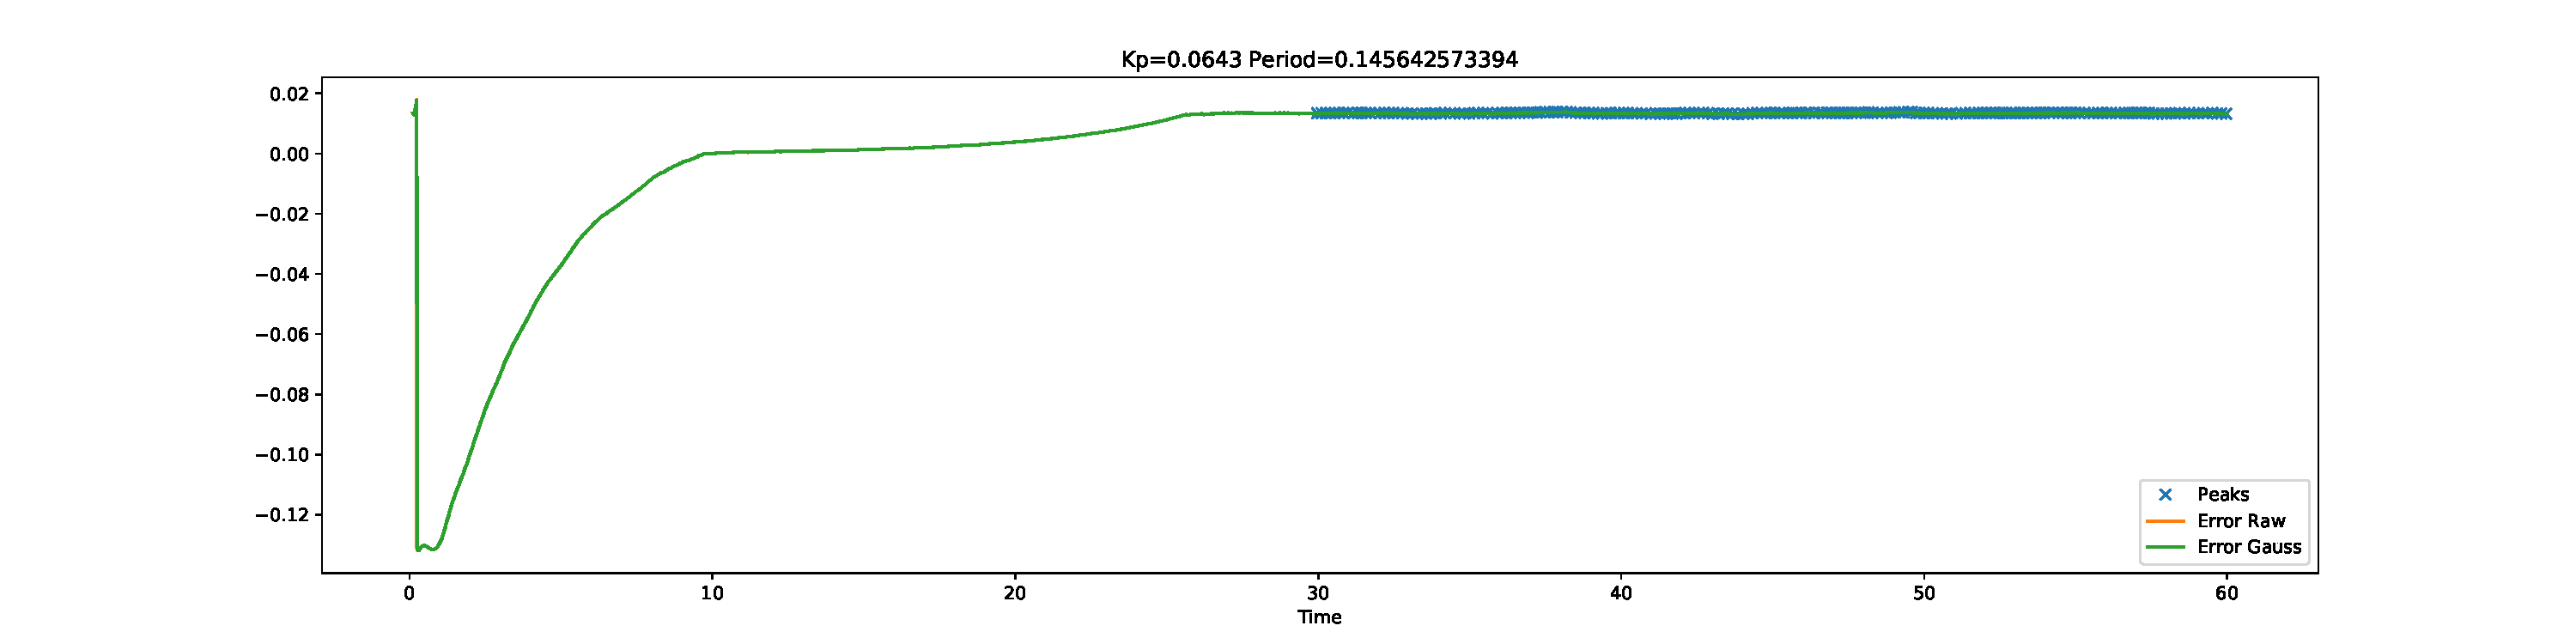
\includegraphics[trim={5cm 0 5cm 0},clip,width=\textwidth]{figures/aeleronTestGain.pdf} 
	\caption{Aileron Ultimate Gain}
\end{figure}

\begin{figure}[ht!] % [h] forces the figure to be output where it is defined in the code (it suppresses floating)
	\centering
	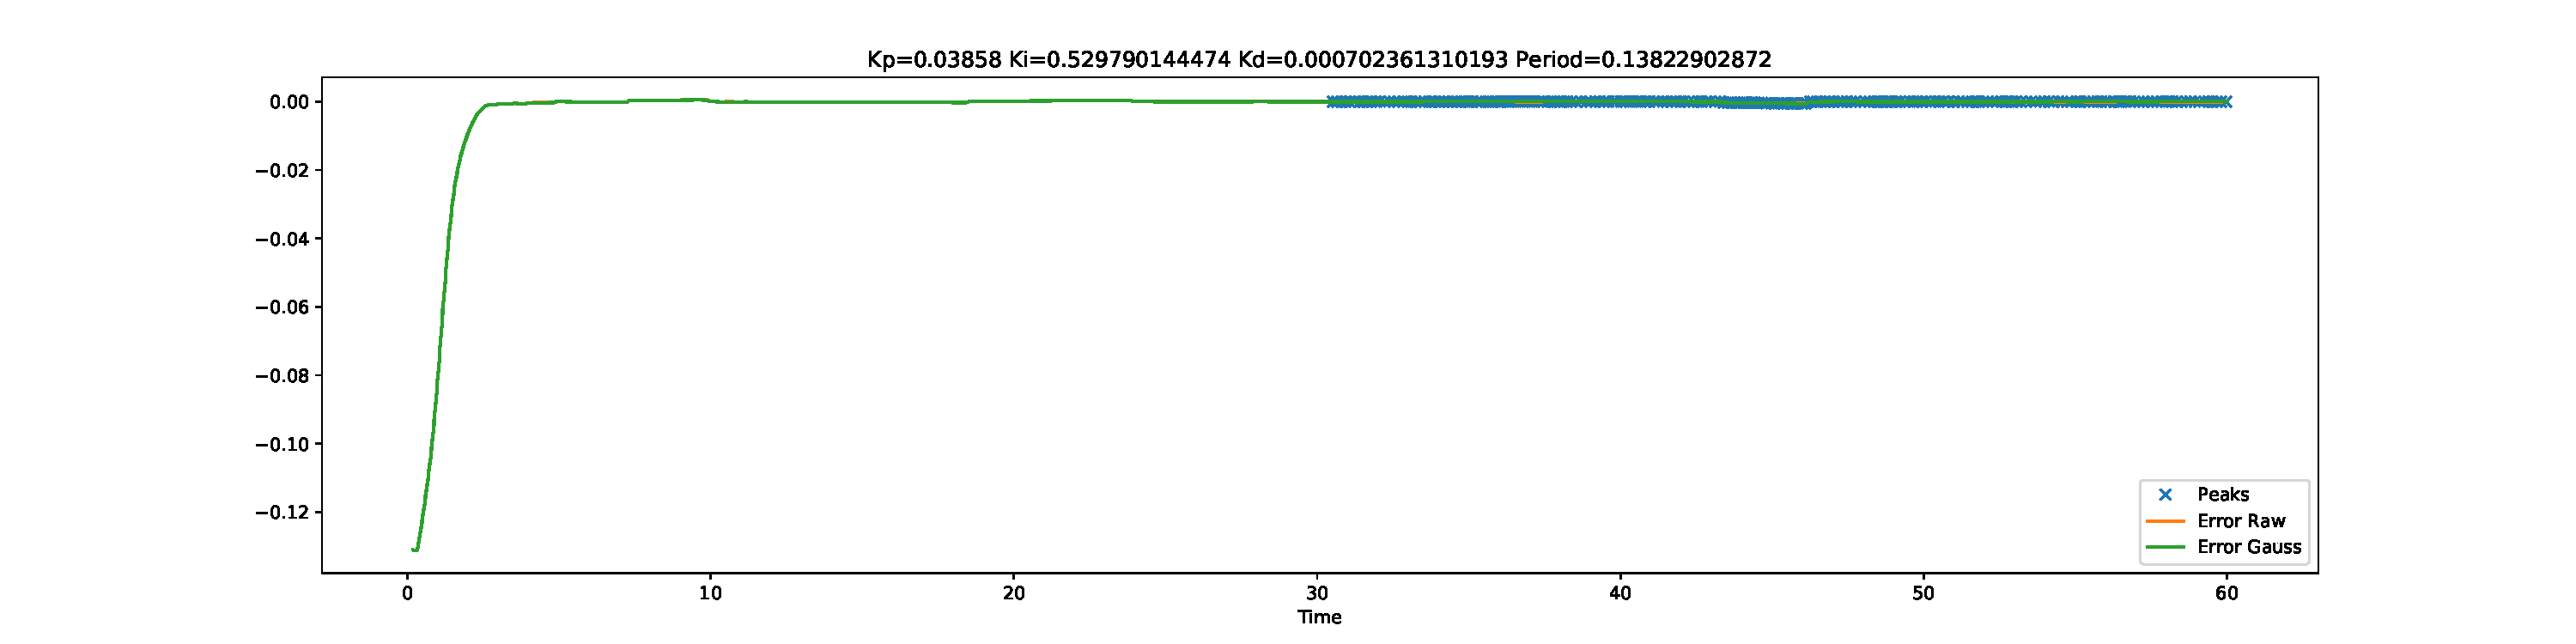
\includegraphics[trim={5cm 0 5cm 0},clip,width=\textwidth]{figures/aeleronZiglerNichols.pdf} 
	\caption{Aileron Ziegler Nichols Test}
\end{figure}


\begin{figure}[ht!] % [h] forces the figure to be output where it is defined in the code (it suppresses floating)
	\centering
	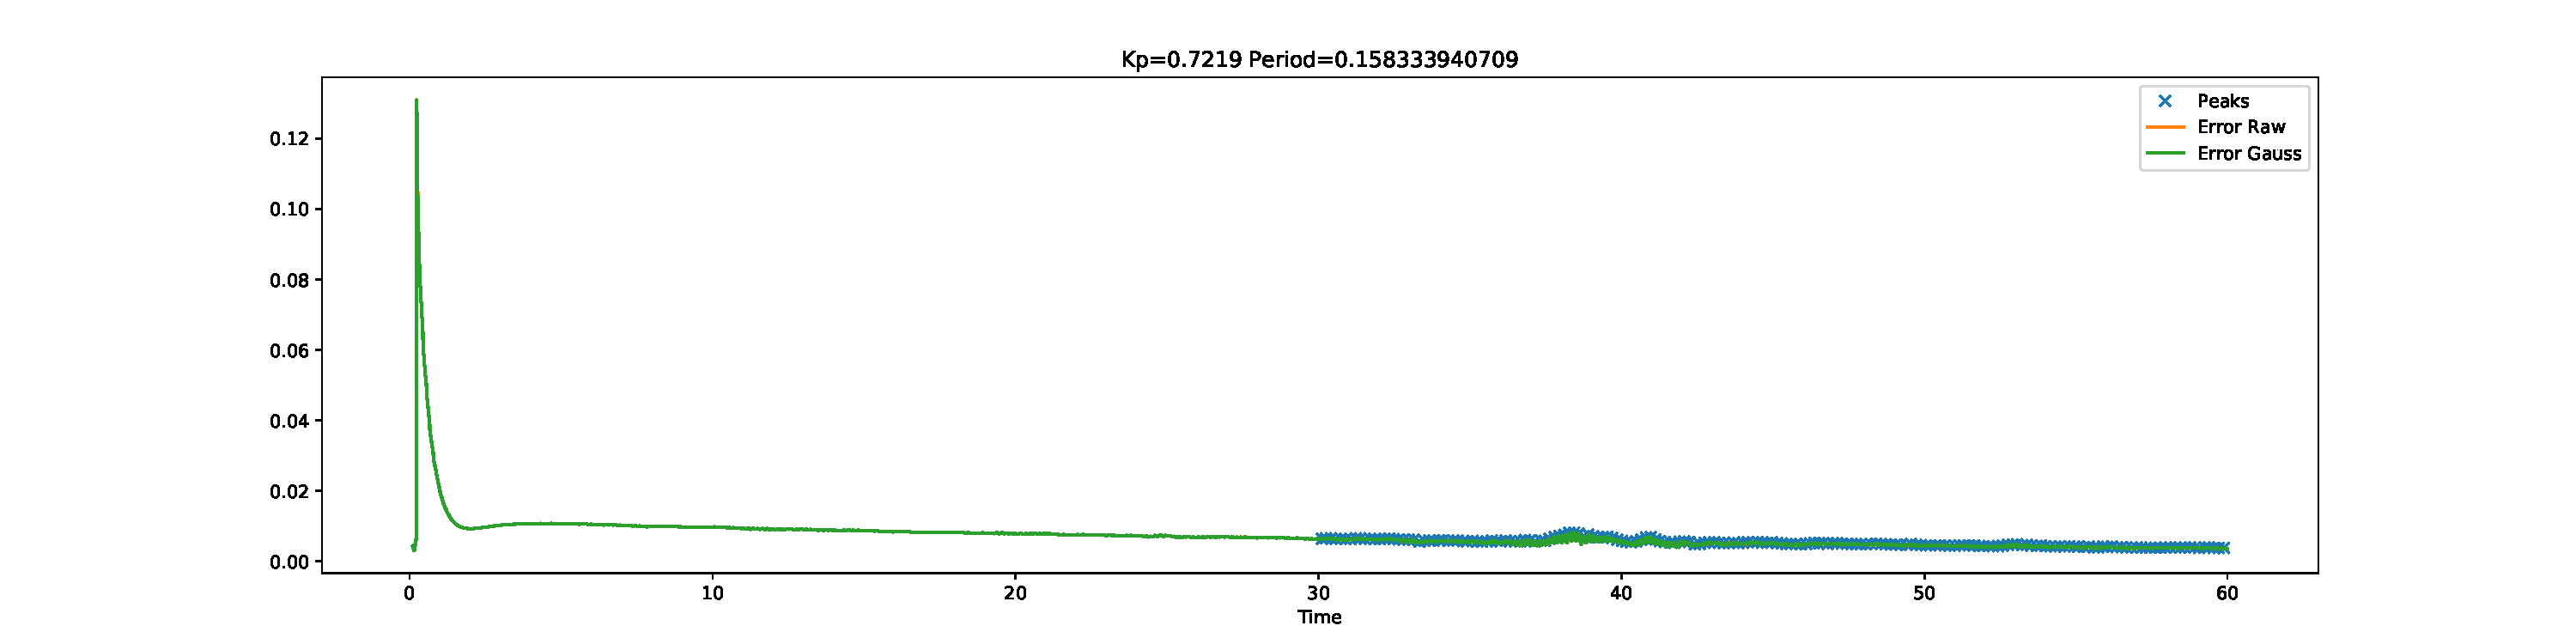
\includegraphics[trim={5cm 0 5cm 0},clip,width=\textwidth]{figures/rudderTestGain.pdf} 
	\caption{Rudder Ultimate Gain}
\end{figure}

\begin{figure}[ht!] % [h] forces the figure to be output where it is defined in the code (it suppresses floating)
	\centering
	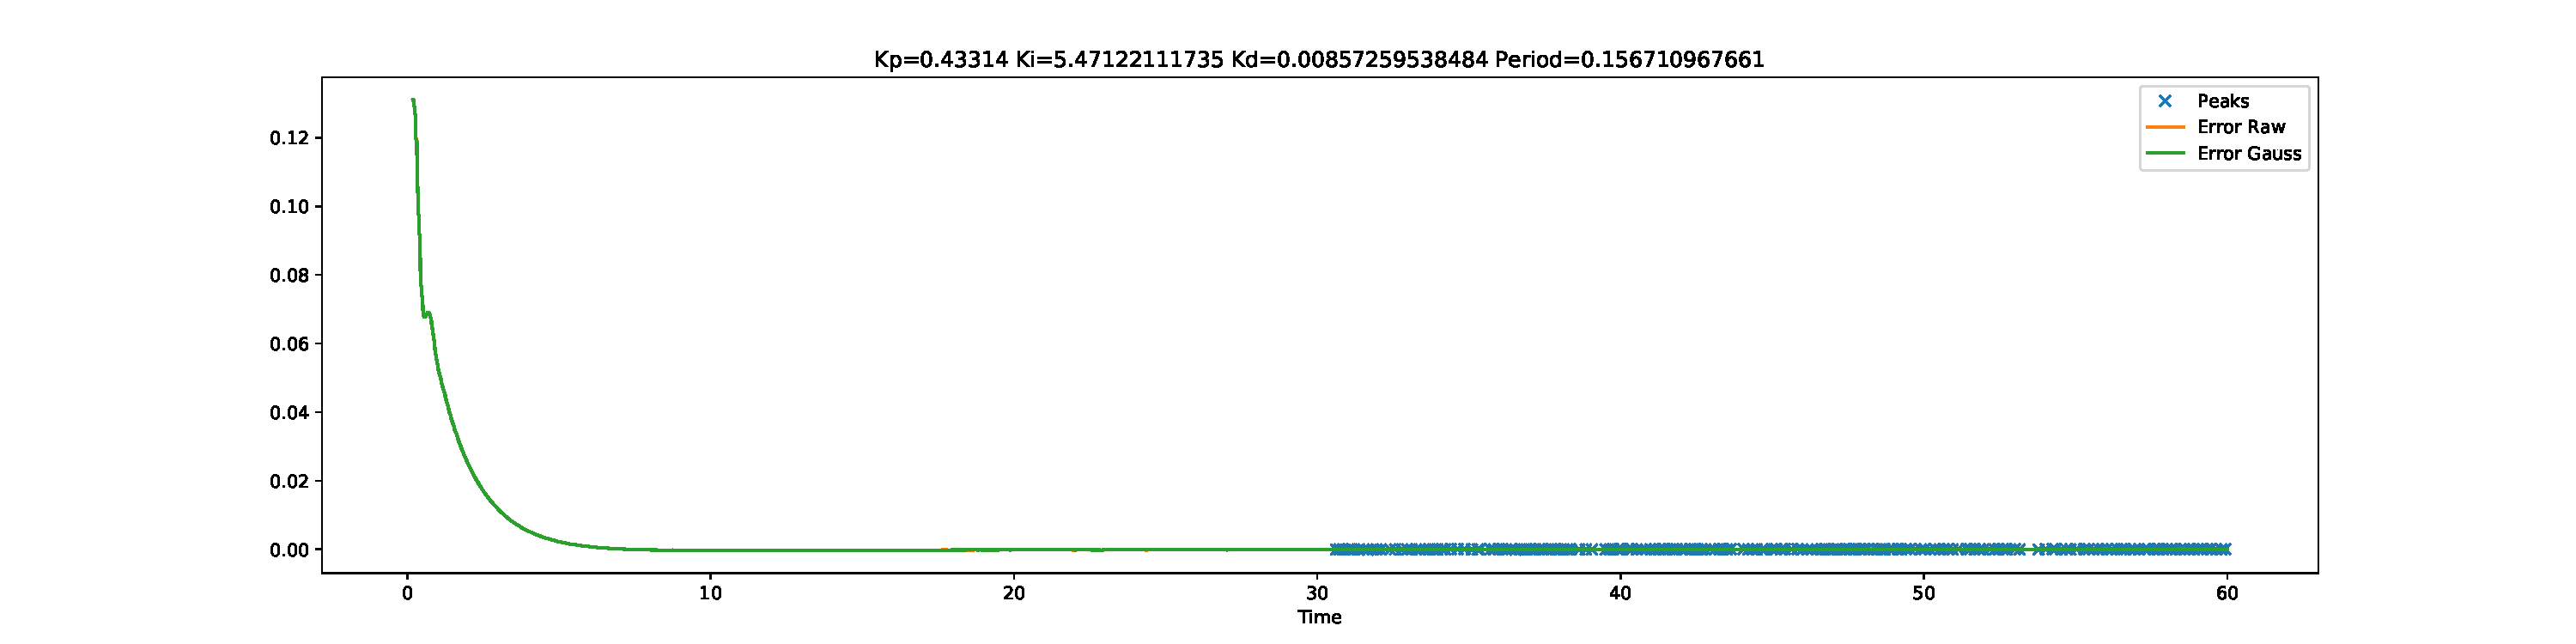
\includegraphics[trim={5cm 0 5cm 0},clip,width=\textwidth]{figures/rudderZiglerNichols.pdf} 
	\caption{Rudder Ziegler Nichols Test}
\end{figure}

\clearpage
\section{Changes to face detection}

When looking through the dataset for my eyebrows I found that about half of the labels for the left and right eyebrows were swapped. This ended up being caused by taking eyebrow samples with two different cameras. The camera on my laptop mirrors the image when capturing while the camera on my desktop computer does not. After re-labeling the images correctly and changing the image format from RGB to gray-scale I got much more accurate model than before.


\begin{figure}[ht!] % [h] forces the figure to be output where it is defined in the code (it suppresses floating)
	\centering
	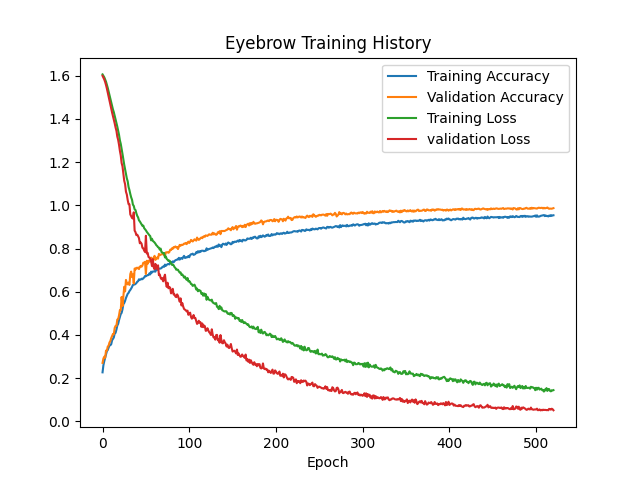
\includegraphics[width=0.8\columnwidth]{figures/trainingGraph.png} 
	\caption{}
\end{figure}

\begin{figure}[ht!] % [h] forces the figure to be output where it is defined in the code (it suppresses floating)
	\centering
	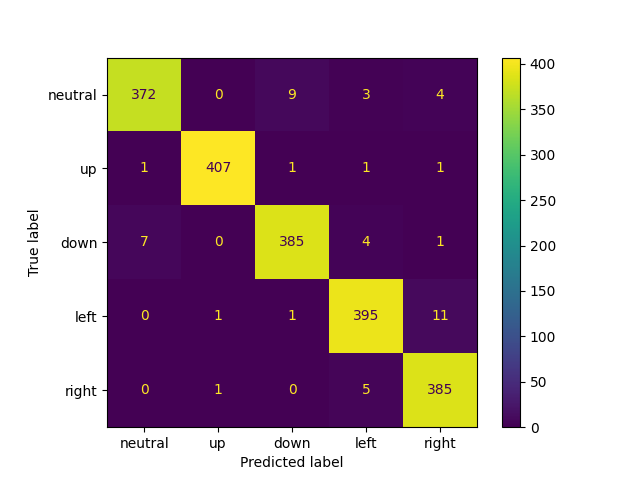
\includegraphics[width=0.49\columnwidth]{figures/confusionMatrixOld.png} 
	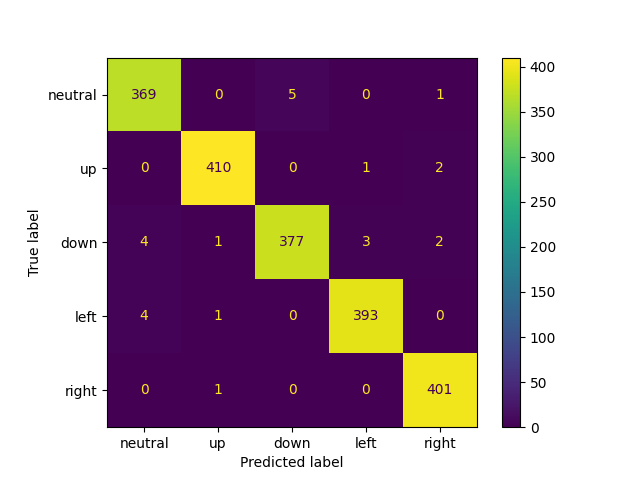
\includegraphics[width=0.49\columnwidth]{figures/confusionMatrix.png} 
	\caption{RGB images with old dataset on left. Greyscale images with new dataset on right.}
\end{figure}

As you can see from the Confusion matricies, the new model no longer mistakes right and left commands. This is what initially tipped me off to the problem as it seemed like right and left should have been visually "opposite" and the least likely to be confused.

\clearpage

\section{Misc Changes}
I made the plane teleport to 10 meters above the ground with a small initial velocity when starting the attitude controller because it helps for testing purposes. The physics simulator takes into account friction and when trying to launch the plane from the ground I would have to max out the plane’s thrust to get it airborne and then decrease it dramatically.
\\

I added a runway world file to the gazebo physics simulator startup to have something more interesting to look at rather than an empty world. It also helps when controlling the aircraft because otherwise there is no visual reference for where it is going. This change was not possible until I moved the virtual machine housing the project to a more powerful computer. The processor was not capable of keeping up with the real-time physics simulations on the old machine when also trying to render anything other than an empty world. 
\\

The service calls to enable and disable the flight controllers and alter their setpoints were changed to topic publications instead. The rates that the information was being published made more sense for the topic topology.
\clearpage


\section{Code}
All files related to this project can be found at:

\url{https://github.com/Trenton-Ruf/Intelligent_Robotics}

\lstinputlisting[
	caption=attitude\_control\_gazebo.py, % Caption above the listing
	%label=lst:test, % Label for referencing this listing
	language=Python, % Use Perl functions/syntax highlighting
	frame=single, % Frame around the code listing
	breaklines=true,
	postbreak=\mbox{\textcolor{red}{$\hookrightarrow$}\space},	
	showstringspaces=false, % Don't put marks in string spaces
	numbers=left, % Line numbers on left
	numberstyle=\tiny, % Line numbers styling
	basicstyle=\footnotesize
	]{../../../catkin_ws/src/rosflight_control/src/attitude_control_gazebo.py}
\clearpage

\lstinputlisting[
	caption=altitude\_control\_gazebo.py, % Caption above the listing
	%label=lst:test, % Label for referencing this listing
	language=Python, % Use Perl functions/syntax highlighting
	frame=single, % Frame around the code listing
	breaklines=true,
	postbreak=\mbox{\textcolor{red}{$\hookrightarrow$}\space},	
	showstringspaces=false, % Don't put marks in string spaces
	numbers=left, % Line numbers on left
	numberstyle=\tiny, % Line numbers styling
	basicstyle=\footnotesize
	]{../../../catkin_ws/src/rosflight_control/src/altitude_control.py}
\clearpage

\lstinputlisting[
	caption=eyebrow\_state\_machine.py, % Caption above the listing
	%label=lst:test, % Label for referencing this listing
	language=Python, % Use Perl functions/syntax highlighting
	frame=single, % Frame around the code listing
	breaklines=true,
	postbreak=\mbox{\textcolor{red}{$\hookrightarrow$}\space},	
	showstringspaces=false, % Don't put marks in string spaces
	numbers=left, % Line numbers on left
	numberstyle=\tiny, % Line numbers styling
	basicstyle=\footnotesize
	]{../../../catkin_ws/src/rosflight_control/src/eyebrow_state_machine.py}
\clearpage

\lstinputlisting[
	caption=faceSocket.py, % Caption above the listing
	%label=lst:test, % Label for referencing this listing
	language=Python, % Use Perl functions/syntax highlighting
	frame=single, % Frame around the code listing
	breaklines=true,
	postbreak=\mbox{\textcolor{red}{$\hookrightarrow$}\space},	
	showstringspaces=false, % Don't put marks in string spaces
	numbers=left, % Line numbers on left
	numberstyle=\tiny, % Line numbers styling
	basicstyle=\footnotesize
	]{../../../faceCNN/faceSocket.py}
\clearpage

\end{document}
